\documentclass{beamer}
\usepackage[utf-8]{inputenc}
\usepackage{graphicx, subfigure}
\usepackage{longtable}
\usepackage{amsmath,amsfonts}
\usepackage{array}
\usepackage{xspace}
\usepackage{color, fancyvrb, relsize}
\usepackage{url, hyperref}
\usepackage{algorithm, algorithmic, listings}
%% \usepackage[francais]{babel}
%% \selectlanguage{francais}

\newcommand{\<}[1]{\`#1}

%ref: http://tex.dante.jp/typo/index.php?Listings#l8795a28

\usepackage{color,graphicx}
%\usepackage[margin=2.5cm]{geometry}
%\usepackage{type1cm}
\usepackage{listings}

\lstdefinelanguage{Scheme}{%
   keywords={begin,call-with-current-continuation,call/cc,%
      call-with-input-file,call-with-output-file,case,cond,do,%
      delay,else,force,for-each,if,lambda,let,let-syntax,let*,%
      letrec,letrec-syntax,and,or,not,map,syntax,syntax-rules,%
      with-mode,with-input-from-file,with-input-fromport,%
      with-output-to-file,with-output-to-port,define,%
			set!, eq?, equal?, eqv?, symbol?, string?, string=?,
			append, string-append, vector-append, string, vector,
			symbol, symbol->string, string->symbol, list, list-ref,
			list-set!, list-tail, set-car!, set-cdr!, car, cdr,
			vector-ref, vector-set!
   },%
   sensitive,%
   alsodigit=-,%
   morecomment=[l]{;},% 
   morecomment=[s]{\#|}{|\#},% 
   morestring=[b]{"}% 
  }[keywords,comments,strings]%"

\lstdefinelanguage[MIT]{Scheme}{%
   morekeywords=[1]{begin,call-with-current-continuation,call/cc,%
      call-with-input-file,call-with-output-file,case,cond,do,%
      delay,else,force,for-each,if,lambda,let,let-syntax,let*,%
      letrec,letrec-syntax,and,or,not,map,syntax,syntax-rules,%
      with-mode,with-input-from-file,with-input-fromport,%
      with-output-to-file,with-output-to-port,define%
   },%
   morekeywords=[2]{fluid-let,%
     in-package,local-declare,macro,make-environment,named-lambda,%
     using-syntax,with-input-from-string,with-output-to-string,%
     with-values,syntax-table-define,list-transform-positive,%
     list-transform-negative,list-search-positive,list-search-negative,%
     access-components,assignment-components,combination-components,%
     comment-components,conditional-components,disjunction-components,%
     declaration-components,definition-components,delay-components,%
     in-package-components,lambda-components,lambda-components*,%
     lambda-components**,open-block-components,pathname-components,%
     procedure-components,sequence-components,unassigned?-components,%
     unbound?-components,variable-components,%
     \#t,\#f,\#e,\#i,\#b,\#o,\#d,\#l,\#s,\#x,\#!\#*,\#@,\#=,\#\#,%
     access,cons-stream,declare,default-object?,define-integrable,%
     define-structure,define-syntax,er-macro-transformer,%
     non-hygienic-macro-transformer,quasiquote,quote,%
     rsc-macro-transformer,sc-macro-transformer,set!,%
     eq?,eqv?,equal?,%
     gcd,modulo,imag-part,numerator,inexact->exact,quotient,abs,%
     lcm,rationalize,angle,magnitude,real-part,ceiling,make-polar,%
     remainder,denominator,make-rectangular,round,expt,max,truncate,%
     floor,min%
  }%
   sensitive=true,%
   alsodigit=-,%
   morecomment=[l]{;},% 
   morecomment=[s]{\#|}{|\#},% 
   morestring=[b]{"}% "
}

\lstset{%
 frame=single,%
 keywordstyle={\ttfamily \color[rgb]{.1, .7, .7}},%
 stringstyle={\ttfamily \color[rgb]{0,.9,0}},%
 commentstyle={\ttfamily \color[rgb]{.9,0,0}},%
 identifierstyle={\color[rgb]{0,0,0}},%
 basicstyle={\ttfamily \color[rgb]{0,0,0}},%
 breaklines=true,%
 columns=[l]{fullflexible},%
 numbers=left,%
 %stepnumber=5,%
 numberstyle={\scriptsize},%
 numbersep=1em,%
 language={Scheme},%
}
\newcommand*\schemesrc[1]{\lstinputlisting[caption={question~#1}]{#1.scm}}



\lstloadlanguages{C,Haskell,Prolog,ML,Lisp,Scheme}
\lstset{language=Scheme}
\lstset{moredelim=*[is][\ttfamily \color{blue}]{|-}{-|}}
%\lstset{moredelim=*[s][\color{red}]{(}{\ }}}

% for themes, etc.
\mode<presentation>
{ \usetheme{boxes} }

\usepackage{times}  % fonts are up to you
\usepackage{graphicx}

% these will be used later in the title page
\title{Space Invaders Development}
\author{David St-Hilaire}
\titlegraphic{
\includegraphics[scale=0.7]{medium-intro}}

\date{August 27, 2008}

% note: do NOT include a \maketitle line; also note that this title
% material goes BEFORE the \begin{document}

% have this if you'd like a recurring outline
\AtBeginSection[]  % "Beamer, do the following at the start of every section"
{
\begin{frame}<beamer> 
\frametitle{Outline} % make a frame titled "Outline"
\tableofcontents[currentsection]  % show TOC and highlight current section
\end{frame}
}

\begin{document}

% this prints title, author etc. info from above
\begin{frame}
\titlepage
\end{frame}

%%%%%%%%%%%%%%%%%%%%%%%%%%%%%%%%%%%%%%%%%%%%%%%%%%%%%%%%%%%%%%%%%%%%%%%%%%%%%%%

\section{Introduction}

\begin{frame}
  \frametitle{Video games in scheme?}
  Why would I want to create video games in scheme?
  \begin{itemize}
  \item Demonstrate the expressiveness of high level languages
  \item Demonstrate a short development cycle
  \item Easily \alert{understandable} and \alert{readable} code
  \item Less bugs
  \item Expermient video game creation with GC
  \end{itemize}
\end{frame}

\begin{frame}
  \frametitle{Why Space Invaders?}

  \begin{columns}[c]
    \begin{column}{7cm} 
      It's a very simple game but it requires:
      \begin{itemize}
      \item real time user interaction
      \item approx. constant screen refresh rate
      \item level development
      \item multiplayer games
      \end{itemize}
    \end{column}
    \begin{column}{5cm} 
\includegraphics[scale=0.5]{medium} \end{column}
  \end{columns}
\end{frame}

\begin{frame}
  \frametitle{Some mertrics}

  \begin{block}{initial development time}
    8 weeks
  \end{block}

  \begin{block}{code size (\# of lines)}
    \begin{itemize}
    \item image reader (ppm): 80
    \item coroutines: 200
    \item discrete event simulation: 280
    \item user interface: 380
    \item fonts and textures: 500 + images
    \item other libraries: 870
    \item opengl, glu, glut interfaces: 1700
    \item \alert{engine: 1800}
    \end{itemize}
  \end{block}
\end{frame}

\begin{frame}
  \frametitle{Architecture}
  \includegraphics[scale=0.7]{arch-en}
\end{frame}


%%%%%%%%%%%%%%%%%%%%%%%%%%%%%%%%%%%%%%%%%%%%%%%%%%%%%%%%%%%%%%%%%%%%%%%%%%%%%%%

\section{Initial version development highlights}

\begin{frame}[fragile]
  \frametitle{Data structures}

  \begin{block}{}
  \begin{itemize}
    \item Usage of gambit's (define-tye ...)
    \item limited object hierarchy
    \item typechecking and dispatch is \alert{hardcoded} :(
  \end{itemize}
  \end{block}

  \begin{block}{exemple}
    \begin{lstlisting}[basicstyle=\footnotesize]
(define-type game-object id type pos state color speed 
  extender: define-type-of-game-object)
(define-type-of-game-object invader-ship row col)
(define-type-of-game-object player-ship)
...
(define types
  `( (easy ,(make-object-type 'easy (make-rect 0 0 12 8) 2 10))
    (medium ,(make-object-type 'medium (make-rect 0 0 12 8) 2 20))
     ..
  ))
    \end{lstlisting}
  \end{block}

\end{frame}



\begin{frame}
  \frametitle{Control flow}
  \begin{block}{Discrete event simulation}
    \begin{itemize}
    \item High level expressiveness
    \item Close to human reasonning
    \item Readily implemented
    \end{itemize}
  \end{block}
\end{frame}

\begin{frame}[fragile]
  \frametitle{Control flow}
  \begin{block}{Exemple}
    \begin{lstlisting}[basicstyle=\footnotesize]
(define (create-mothership-event level)
 (define mothership-event
   (lambda ()
     (let ((mothership (level-mothership level)))
       (if mothership
           (let ((collision-occured? (move-object! level mothership)))
             (if (or (not collision-occured?)
                     (is-explosion? collision-occured?))
                 (in mothership-update-interval mothership-event)))))))
 mothership-event)

(in 1.5 (create-mothership-event level))
    \end{lstlisting}
  \end{block}
\end{frame}

\begin{frame}
  \frametitle{UI and Engine decoupling}

  Both UI and the engine are ran seperatly in gambit threads
  \begin{block}{User Interface}
    \begin{itemize}
    \item Passive waiting of \texttt{redraw} commands
    \item User input callbacks redirected to the engine
    \end{itemize}
  \end{block}

  \begin{block}{Engine}
    \begin{itemize}
    \item frequently polls the UI for user inputs
    \item periodically sends \texttt{redraw} commands to UI
    \item Completely independant of the UI
    \end{itemize}
  \end{block}
\end{frame}

\begin{frame}
  \frametitle{Pause}

  \begin{block}{Discrete event simulation semaphores }
    \begin{itemize}
      \item Event's continuation stored in a waiting queue
    \end{itemize}
  \end{block}

  \begin{block}{\texttt{synchronized-event-thunk} macro}
    \begin{itemize}
      \item Runs an event inside a fake critical sections
      \item Makes easy the seperation of what will get paused
    \end{itemize}
  \end{block}

  \begin{block}{Other usages}
    \begin{itemize}
      \item Pause is used to create specific animation effects
    \end{itemize}
  \end{block}
\end{frame}


\begin{frame}
  \frametitle{Animations}
  \begin{itemize}
  \item Easily represented as recursive events
  \item Usage of an extra parameter: \alert{continuation} event!
  \item Good modularity of animation events
  \end{itemize}
\end{frame}

\begin{frame}[fragile]
  \frametitle{Animations}
  \begin{block}{Exemple}
    \begin{lstlisting}[basicstyle=\footnotesize]
(in 0 (animate-message
           (level-get level 'mother) "=? MYSTERY"
           (animate-message
            (level-get level 'hard) "=30 POINTS"
            (animate-message
             (level-get level 'medium) "=20 POINTS"
             (animate-message
              (level-get level 'easy) "=10 POINTS"
              (lambda ()
                (in animation-end-wait-delay ...
    \end{lstlisting}
  \end{block}
\end{frame}

\begin{frame}
  \frametitle{Collision detection and response}

  Collision detection and response is integrated into object movement.

  \begin{block}{Detection}
    \begin{itemize}
    \item Rectangle to Rectangle (\textit{bounding-box})
    \item Point to Rectangle
    \end{itemize}
  \end{block}

  \begin{block}{Response}
    \begin{itemize}
    \item Based on the colliding object's \alert{type}
    \item Manual dispatch of collision response :(
    \item Multiple models are used: (objets, point clouds)
    \end{itemize}
  \end{block}
\end{frame}


\begin{frame}
  \frametitle{Multiplayer games}

  \begin{block}{Coroutines}
    \begin{itemize}
    \item Cooperative threads with explicit context switch
      (\texttt{yield})
    \item Inter-coroutine messaging system (\texttt{!}, \texttt{?})
    \end{itemize}
  \end{block}

  \begin{block}{Usage}
    \begin{itemize}
    \item Each player runs in its own coroutine
    \item The \texttt{yield} operation enables to switch between players
    \item Some events must be pre-scheduled 
    \end{itemize}
  \end{block}
\end{frame}

\begin{frame}
  \frametitle{Graphical rendering}
  
  \begin{itemize}
  \item Need to easily render sprites
  \item Must be able to read and load image files
  \item Must efficiently render sprites
  \end{itemize}

  \begin{block}{}
    \begin{columns}[c]
      \begin{column}[c]{2cm}
        
\includegraphics[scale=0.2]{easy0}
      \end{column}
      \begin{column}[c]{2cm}
        
\includegraphics[scale=0.2]{easy1}
      \end{column}
    \end{columns}
  \end{block}

\end{frame}

\begin{frame}
  \frametitle{Graphical rendering}
  \begin{block}{Idea}
    \begin{itemize}
    \item Combination of smaller semantically related images
    \item Runtime image loading
    \item Optionnal compile-time image loading
    \item Usage of opengl textures
    \end{itemize}
  \end{block}
  
  \begin{block}{Problem}
    \begin{itemize}
    \item Texture resize is expansive
    \end{itemize}
  \end{block}
\end{frame}

\begin{frame}[fragile]
  \frametitle{Graphical rendering}

  \begin{block}{Exemple}
    \begin{center}
      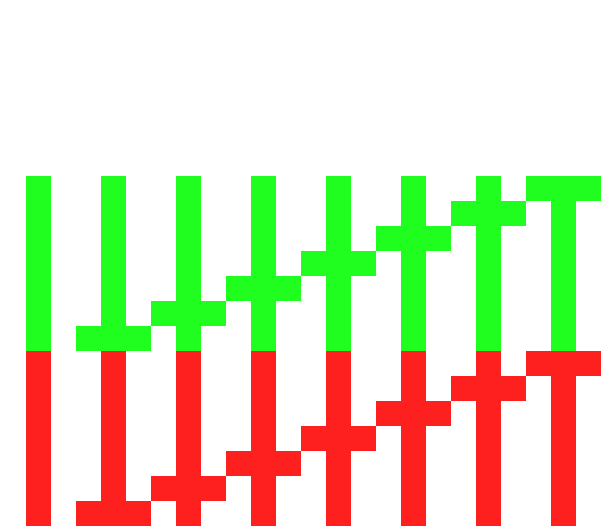
\includegraphics[scale=0.2]{font-exemple}
    \end{center}
    \begin{lstlisting}[basicstyle=\footnotesize]
((colors: (white green red))
 (chars: (0 1 2 3 4 5 6 7)))
    \end{lstlisting}
  \end{block}
\end{frame}


%%%%%%%%%%%%%%%%%%%%%%%%%%%%%%%%%%%%%%%%%%%%%%%%%%%%%%%%%%%%%%%%%%%%%%%%%%%%%%%


\section{Improvements}

\begin{frame}
  \frametitle{Portability}
  \begin{block}{mac-os portability}
    \begin{itemize}
    \item Readily achieved throught the framework system
    \item Only small makefile tweeks were required
    \end{itemize}
  \end{block}

  \begin{block}{window portability}
    \begin{itemize}
    \item Very troublesome! Glut never worked under windows...
    \item Switched the UI to SDL
    \item Finally compiled under mingw
    \end{itemize}
  \end{block}
\end{frame}

\begin{frame}
  \frametitle{Object system and automatic dispatch}

  \begin{block}{Requirements}
    \begin{itemize}
    \item fast member access
    \item class members
    \item virtual classes?
    \item multiple dispatch (polymorphism)
    \item multiple inheritane
    \end{itemize}
  \end{block}

\end{frame}

\begin{frame}
  \frametitle{Object system and automatic dispatch: OOPS}

  \begin{block}{OOPS}
    \begin{itemize}
    \item Nice and very vast clos-like object system
    \item Fullfills most of the requirements
    \item Leads to very nice code
    \item Runs very \alert{slowly} (approx 1-2 FPS)... :(
    \end{itemize}
  \end{block}

\end{frame}

\begin{frame}[fragile]
  \frametitle{Object system and automatic dispatch: OOPS}

  \begin{block}{Exemple: Class declarations}
    \begin{lstlisting}[basicstyle=\tiny]
(define-class <game-object>      () ( (:id) (:pos) ))
(define-class <statefull-object> () (:state))
(define-class <colored-object>   () (:color))
(define-class <movable-object>   () (:speed))
(define-class <sprite-object> (<game-object>
                                <statefull-object>
                                <colored-object>)
  ())
(define-class <invader> (<sprite-object>
                         <movable-object>
                         <valuable-object>)
  ((:row)
   (:col)))

(define-class <easy> (<invader>)
  ((:class-id    allocation: class: init-value: 'easy)
   (:bbox        allocation: class: 
          init-value: (<rect> :x: 0 :y: 0
                               :width: 12 :height: 8))
   (:state-num   allocation: class: init-value: 2)
   (:score-value allocation: class: init-value: 10)))
    \end{lstlisting}
  \end{block}

\end{frame}


\begin{frame}[fragile]
  \frametitle{Object system and automatic dispatch: OOPS}

  \begin{block}{Exemple: Multiple dispatch}
    \begin{lstlisting}[basicstyle=\scriptsize]
(define-method (resolve-collision! level (laser <laser>) (player <player>))
  (explode-player! level player)
  (destroy-laser! level laser))

(define-method (resolve-collision! level (laser <laser>) (shield <shield>))
  (let ((penetrated-pos (get-laser-penetration-pos laser)))
    (:pos-set! laser penetrated-pos)
    (explode-laser! level laser)
    (shield-explosion! shield laser))
  (destroy-laser! level laser))

(define-method (resolve-collision! level (laser <laser>) (mothership <mothership>))
  (destroy-laser! level laser)
  (explode-mothership! level mothership)
  (level-increase-score! level mothership)
  (let ((delta-t (mothership-random-delay)))
    (in delta-t (create-new-mothership-event level))))
    \end{lstlisting}
  \end{block}
\end{frame}

\begin{frame}
  \frametitle{Thread simulation}

  \begin{block}{idea}
    \begin{itemize}
    \item Simplify the architecture: Only use coroutines
    \item Must support scheduler \alert{nesting}
    \item Will hopefully simplify the way events were previously written
    \end{itemize}
  \end{block}
\end{frame}

\begin{frame}
  \frametitle{Thread simulation: API overview}
  \begin{block}{Coroutine creation}
    \begin{itemize}
    \item \texttt{(new-coroutine id thunk)}
    \end{itemize}
  \end{block}

  \begin{block}{Coroutine inter-communication}
    \begin{itemize}
    \item \texttt{(empty-mailbox? corout)}
    \item \texttt{(?)}
    \item \texttt{(! corout msg)}
    \end{itemize}
  \end{block}

  \begin{block}{Coroutine control flow}
    \begin{itemize}
    \item \texttt{(yield)}
    \item \texttt{(super-yield)}
    \item \texttt{(terminate-corout ret-val)}
    \item \texttt{(spawn-brother corout)}
    \end{itemize}
  \end{block}

\end{frame}


\begin{frame}
  \frametitle{Thread simulation: API overview}
  \begin{block}{Scheduler operations}
    \begin{itemize}
    \item \texttt{(simple-boot corout1 . corouts)}
    \item \texttt{(boot return-val-handler c1 . cs)}
    \item \texttt{(kill-all! ret-val)}
    \end{itemize}
  \end{block}

  \begin{block}{Synchronization}
    \begin{itemize}
    \item \texttt{(sleep-until contition-thunk)}
    \item \texttt{(sleep-for secs)}
    \item \texttt{(new-semaphore init-value)}
    \item \texttt{(sem-locked? sem)}
    \item \texttt{(sem-lock! sem)}
    \item \texttt{(sem-unlock!sem)}
    \end{itemize}
  \end{block}

\end{frame}

\begin{frame}
  \frametitle{Thread simulation: API overview}

  \begin{block}{Macros}
    \begin{itemize}
    \item \texttt{(continue-with-thunk! continuation-thunk)}
    \item \texttt{(prioritized-thunk-continuation continuation-thunk)}
    \item \texttt{(compose-thunks . thunks)}
    \item \texttt{(dynamic-corout-extent before-thunk body-thunk after-thunk)}
    \end{itemize}
  \end{block}

\end{frame}


\begin{frame}[fragile]
  \frametitle{Thread simulation: Usage exemple}
  \begin{block}{Exemple 1: Animation coroutine}
    \begin{lstlisting}[basicstyle=\footnotesize]
(define (player-explosion-animation level expl-obj duration)
  (define frame-rate 0.1)
  (lambda ()
    (let loop ((dt 0))
      (cycle-state! expl-obj)
      (if (< dt duration)
          (begin (sleep-for frame-rate)
                 (loop (+ dt frame-rate)))
          (level-remove-object! level expl-obj)))))
    \end{lstlisting}
    \end{block}
\end{frame}

\begin{frame}[fragile]
  \frametitle{Thread simulation: Usage exemple}
  \begin{block}{Exemple 2: Animation enhanced modularity}
    \begin{lstlisting}[basicstyle=\footnotesize]
(define (create-animate-score-adv-table level)
  ... some objects creation ...
   (continue-with-thunk!
     (compose-thunks
      (animate-message (level-get level 'mother) "=? MYSTERY")
      (animate-message (level-get level 'hard) "=30 POINTS")
      (animate-message (level-get level 'medium) "=20 POINTS")
      (animate-message (level-get level 'easy) "=10 POINTS")
      (lambda ()
        (sleep-for animation-end-wait-delay)
        (continue-with-thunk!
         (lambda ()
           (set! other-animations-index
                 (modulo (+ other-animations-index 1)
                         (length other-animations)))
           (kill-all!
            (list-ref other-animations
                      other-animations-index))))))))
    \end{lstlisting}
    \end{block}
\end{frame}

\begin{frame}
  \frametitle{Current Architecture}
  \begin{block}{1 Player Architecture}
    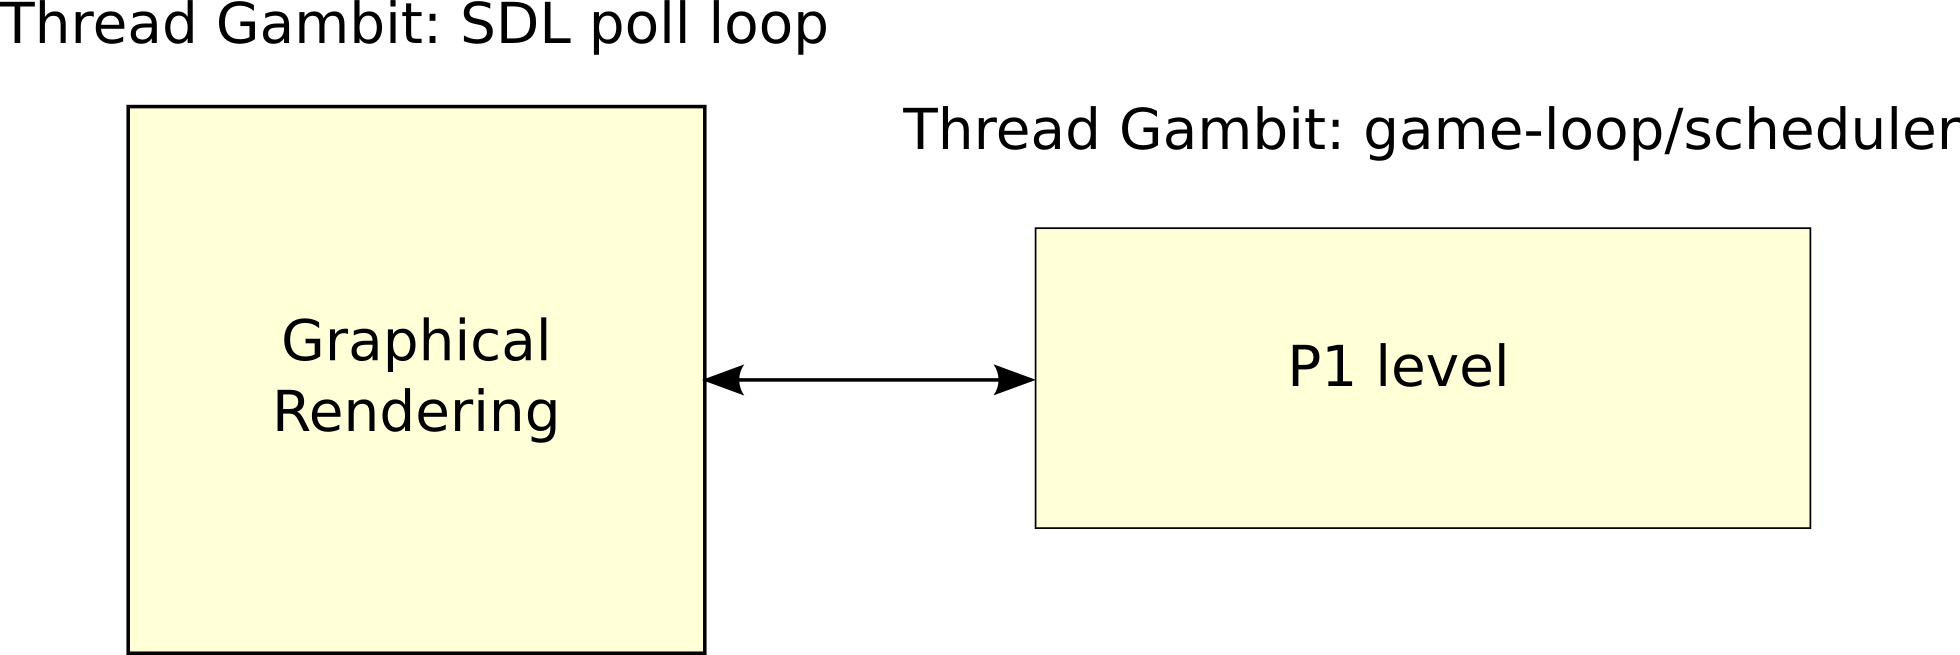
\includegraphics[scale=0.5]{arch-recent-1p}
  \end{block}

  \begin{block}{2 Players Architecture}
    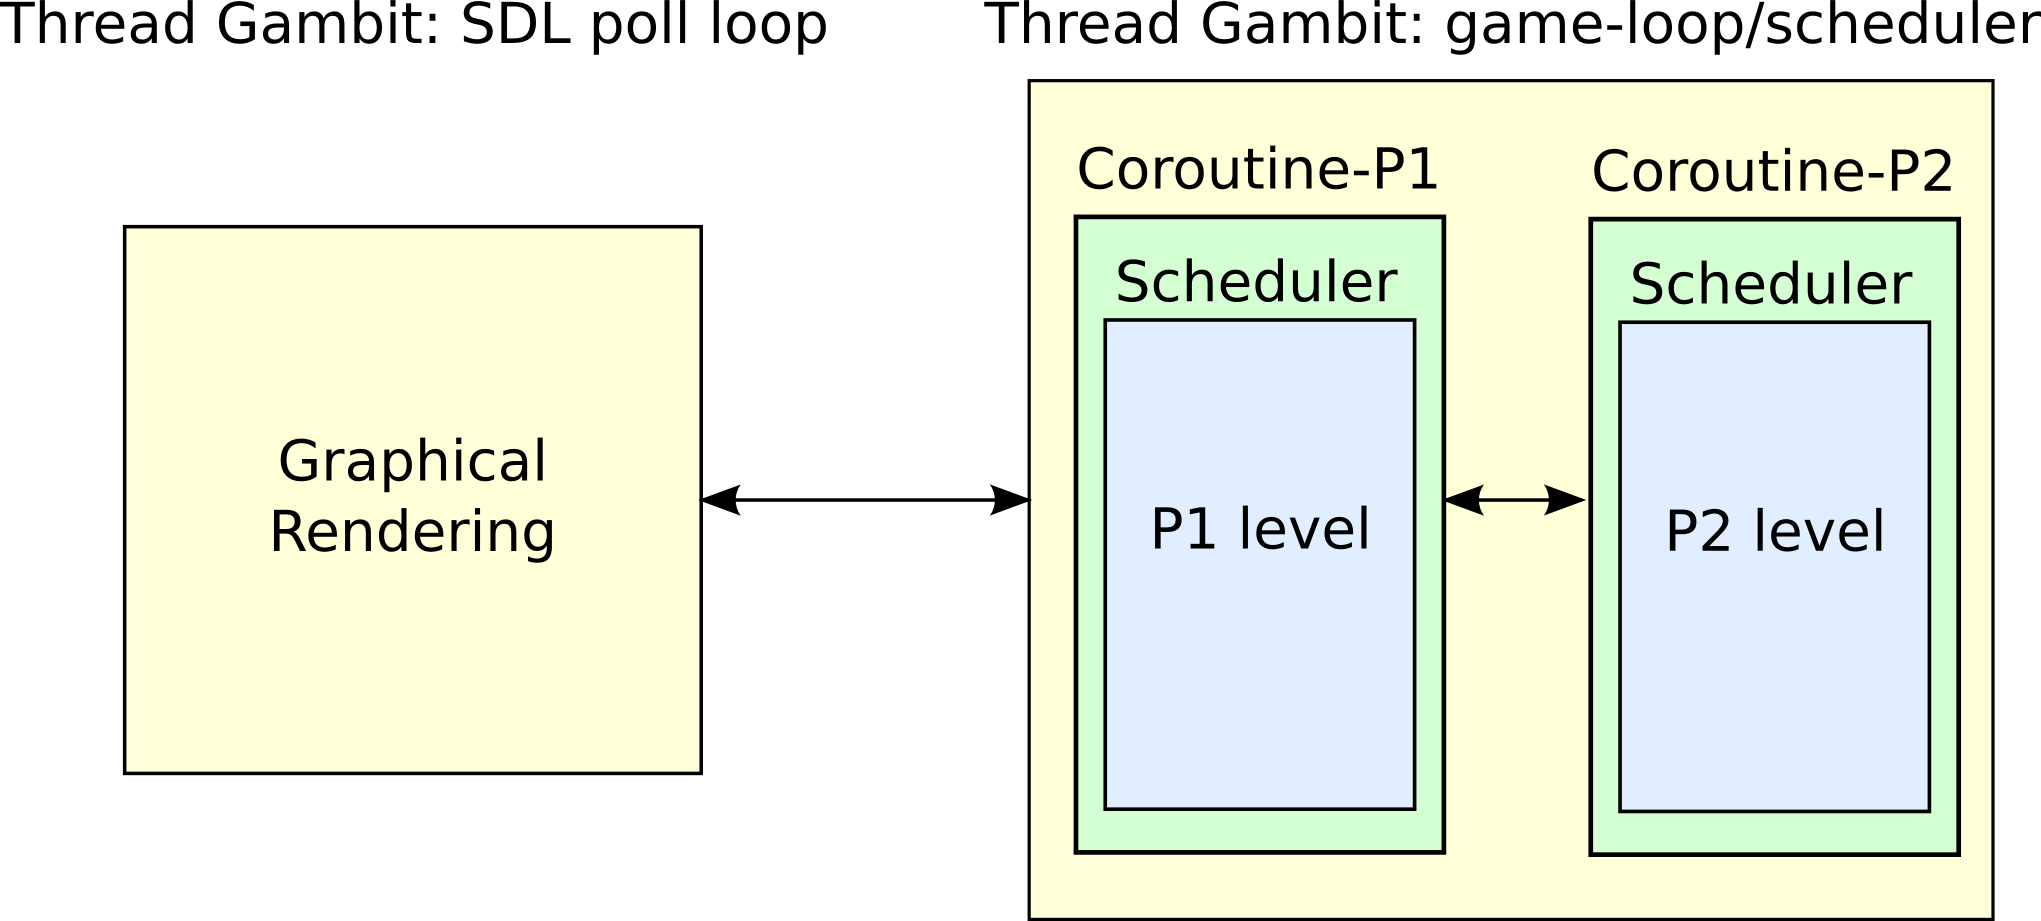
\includegraphics[scale=0.5]{arch-recent-2p}
  \end{block}
\end{frame}


%%%%%%%%%%%%%%%%%%%%%%%%%%%%%%%%%%%%%%%%%%%%%%%%%%%%%%%%%%%%%%%%%%%%%%%%%%%%%%%

\section{What's next?}

\begin{frame}
  \frametitle{Object system module}

  \begin{block}{Differences}
    \begin{itemize}
    \item Must be \alert{fast}
    \item Must support multiple dispatch over generic functions
    \item Must lead to better code (multiple inheritance, class
      members and virtual classes would help!)
    \end{itemize}
  \end{block}

  \begin{block}{Schemer's philosophy}
    \begin{itemize}
    \item If you need something specific and no one else did it
      before, then just do it yourself!
    \end{itemize}
  \end{block}
\end{frame}

\begin{frame}
  \frametitle{Thank You!}
  \begin{center}
    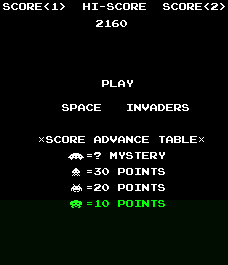
\includegraphics[scale=0.4]{intro-movie2}
  \end{center}
  Thank you for listening! I hope you enjoy the game! :D
\end{frame}


\end{document}
